\documentclass[border=10pt]{standalone}
\usepackage{tikz}
\usetikzlibrary{arrows.meta, positioning, shapes.geometric, calc}

\definecolor{capblue}{HTML}{4A90D9}
\definecolor{threatred}{HTML}{E74C3C}
\definecolor{countergreen}{HTML}{27AE60}
\definecolor{govpurple}{HTML}{8E44AD}
\definecolor{futureorange}{HTML}{F39C12}
\definecolor{introblack}{HTML}{2C3E50}

\begin{document}
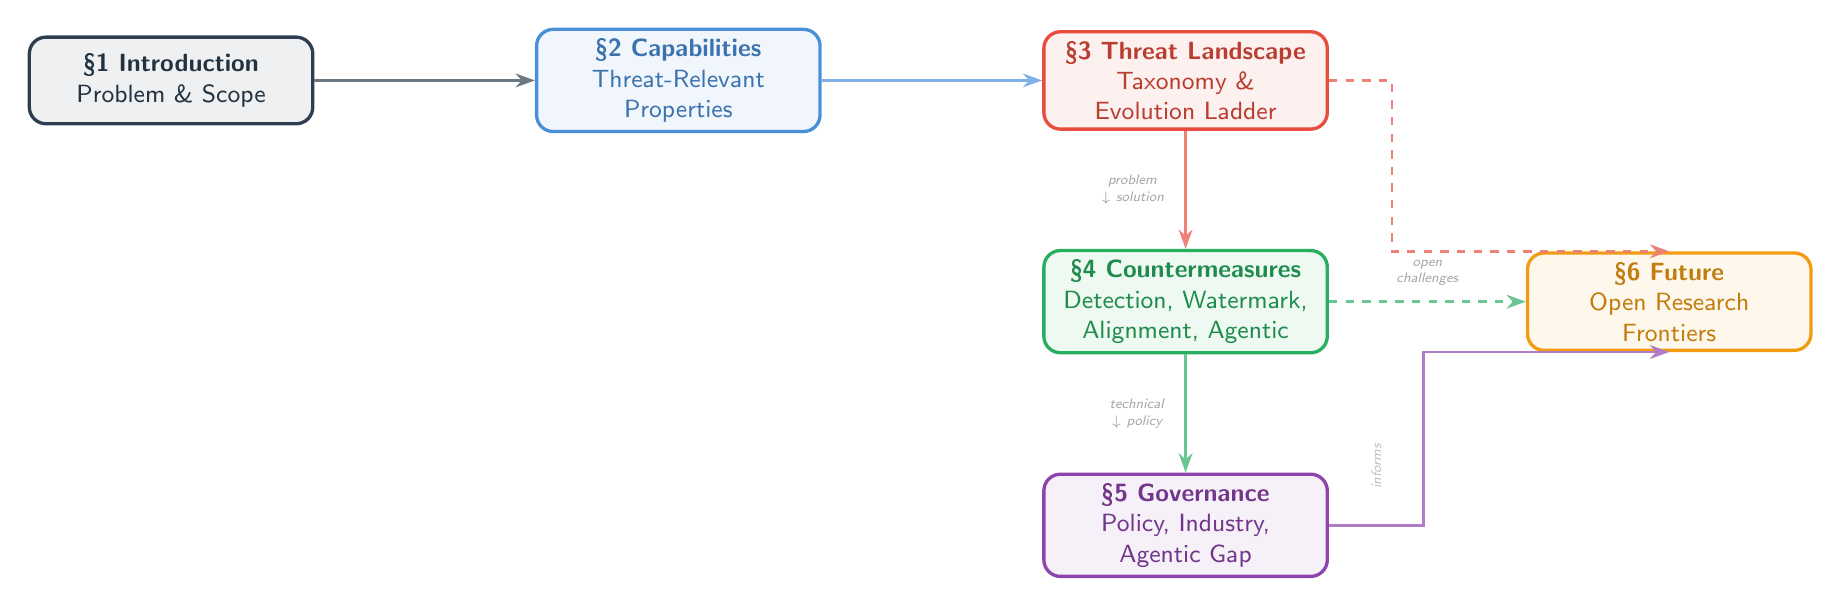
\begin{tikzpicture}[
    node distance=1.8cm and 2.8cm,
    block/.style={
        rectangle, rounded corners=6pt,
        draw=#1, line width=1.2pt, fill=#1!8,
        minimum width=3.6cm, minimum height=1.1cm,
        font=\sffamily\small, align=center, text=#1!80!black
    },
    arrow/.style={-{Stealth[length=7pt,width=5pt]}, line width=1pt, color=#1!70},
    label/.style={font=\sffamily\tiny\itshape, color=gray!70, align=center}
]

% Nodes
\node[block=introblack] (intro) {\textbf{\S1 Introduction}\\Problem \& Scope};

\node[block=capblue, right=of intro] (cap) {\textbf{\S2 Capabilities}\\Threat-Relevant\\Properties};

\node[block=threatred, right=of cap] (threat) {\textbf{\S3 Threat Landscape}\\Taxonomy \&\\Evolution Ladder};

\node[block=countergreen, below=1.5cm of threat] (counter) {\textbf{\S4 Countermeasures}\\Detection, Watermark,\\Alignment, Agentic};

\node[block=govpurple, below=1.5cm of counter] (gov) {\textbf{\S5 Governance}\\Policy, Industry,\\Agentic Gap};

\node[block=futureorange, right=2.5cm of counter] (future) {\textbf{\S6 Future}\\Open Research\\Frontiers};

% Main flow arrows
\draw[arrow=introblack] (intro) -- (cap);
\draw[arrow=capblue] (cap) -- (threat);
\draw[arrow=threatred] (threat) -- (counter) node[label, midway, left=4pt] {problem\\$\downarrow$ solution};
\draw[arrow=countergreen] (counter) -- (gov) node[label, midway, left=4pt] {technical\\$\downarrow$ policy};
\draw[arrow=govpurple] (gov.east) -- ++(1.2,0) |- (future.south) node[label, near start, below=2pt] {};

% Diagonal connection: threat -> future
\draw[arrow=threatred, dashed] (threat.east) -- ++(0.8,0) |- (future.north);

% Counter -> future
\draw[arrow=countergreen, dashed] (counter) -- (future) node[label, midway, above=2pt] {open\\challenges};

% Feedback label
\node[font=\sffamily\tiny\itshape, color=gray!50, rotate=90] at ($(gov.east)+(0.6, 0.75)$) {informs};

\end{tikzpicture}
\end{document}
